The total dissipation of power is composed of two major parts: dynamic and static.
The influence of process variation on the dynamic power is known to be negligibly small \cite{srivastava2010, juan2011, juan2012}; on the other hand, the variability of the static power is substantial, in which the subthreshold leakage current contributes the most \cite{juan2011, juan2012}.
Hence, we shall focus on the subthreshold leakage and, more specifically, on the effective channel length, denoted by $\Leff(\o)$, since it has the strongest influence on leakage and is severely deteriorated by process variation \cite{chandrakasan2001}.
In particular, $\Leff(\o)$ also affects other leakage-magnifying parameters such as the threshold voltage \cite{juan2011}.

It is well-known that the dispersion, due to process variation, of the effective channel length around the nominal value resembles a bell shape similar to the one inherent to Gaussian distributions.
Therefore, such variations are often conveniently modeled using Gaussian random variables \cite{srivastava2010, juan2011, juan2012, chandra2010, shen2009, bhardwaj2006, ghanta2006}.
In this work, due to both the underlying physics and demonstration purposes, we would like to make a step further.
Specifically, we shall bake right into the model the fact that the effective channel length, occupying the space between the drain and source of a nanoscopic transistor, cannot be, say, one meter or take a negative value as Gaussian distributions allow it to do.
To this end, we propose modeling physically-bounded parameters using the four-parametric family of beta distributions: $\dBeta(\alpha, \beta, a, b)$ where $\alpha$ and $\beta$ are the shape parameters, and $a$ and $b$ are the left and right bounds of the support, respectively.
$\alpha$ and $\beta$ can be chosen in such a way that the typically observed bell shape of the distribution is preserved.
An illustration of this technique is given in \fref{beta-normal} where we fitted a beta distribution to the standard Gaussian distribution.
It can be seen that the curves are nearly indistinguishable, but the beta one has a strictly bounded support $[-4, 4]$, which potentially leads to more realistic models.

\begin{figure}[t]
  \centering
  \updatedFigure{
  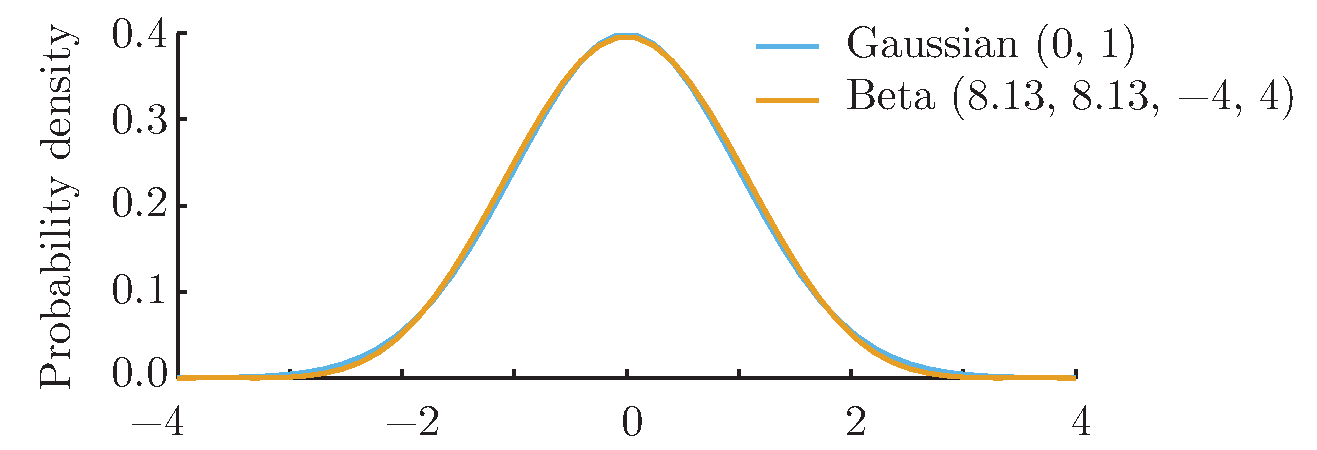
\includegraphics[width=0.9\linewidth]{include/assets/beta-normal.pdf}
  }
  \vspace{-0.5em}
  \caption{The standard Gaussian distribution and a fitted beta distribution.}
  \flabel{beta-normal}
  \vspace{-1.5em}
\end{figure}

The variations of $\Leff(\o)$ are split into global $\gLeff(\o)$ and local $\lLeff(\o)$ parts \cite{chandra2010, shen2009}.\footnote{Without loss of generality, $\gLeff(\o)$ can be treated as a composition of independent inter-lot, inter-wafer, and inter-die variations; likewise, $\lLeff(\o)$ can treated as a composition of independent (purely random) and dependent (spatially correlated) local variations.}
$\gLeff(\o)$ is assumed to be shared among all the $\nvars$ processing elements whereas each processing element has its own local parameter $\lLeff_i(\o)$.
Therefore, the effective channel length $\Leff_i(\o)$ of the $i$th processing element on the die is modeled as follows:
\begin{equation} \elabel{leakage-partition}
  \Leff_i(\o) = \nLeff + \gLeff(\o) + \lLeff_i(\o)
\end{equation}
where $\nLeff$ is the nominal value of the channel length. Consequently, the uncertain parameters of the problem are
\begin{equation} \elabel{uncertain-parameters}
  \vU(\o) = \vec{\lLeff_1(\o), \dotsc, \lLeff_\nprocs(\o), \gLeff(\o) }.
\end{equation}

Global variations are typically assumed to be uncorrelated with respect to the local ones.
The latter, however, are known to have high spatial correlations, which we shall model using the following correlation function:
\begin{align}
  \oCorr{\lLeff_i(\o), \lLeff_j(\o)} \elabel{correlation-function} &= \eta \; \fCorr_\SE(\r_i, \r_j) \\
  & { } \;\;\;\;\; + (1 - \eta) \fCorr_\OU(\r_i, \r_j) \nonumber
\end{align}
where $\r_i \in \real^2$ is the spatial location of the center of the $i$th processing element on the die relative to the center of the die. The correlation function is a composition of two kernels:
\begin{align*}
  & \fCorr_\SE(\r_i, \r_j) = \exp\left(-\frac{\norm{\r_i - \r_j}^2}{\ell_\SE^2}\right) \text{ and} \\
  & \fCorr_\OU(\r_i, \r_j) = \exp\left(- \frac{\abs{\,\norm{\r_i} - \norm{\r_j}\,}}{\ell_\OU} \right),
\end{align*}
which are known as the squared exponential and Ornstein-Uhlenbeck kernels, respectively.
In the above equations, $\eta \in [0, 1]$ is a weighting coefficient balancing the kernels; $\ell_\SE$ and $\ell_\OU > 0$ are so-called length-scale parameters; and $\norm{\cdot}$ stands for the Euclidean distance.
The choice of the correlation function in \eref{correlation-function} is guided by the observations of the correlation structures induced by the fabrication process \cite{chandrakasan2001, friedberg2005, cheng2011}: $\fCorr_\SE$ imposes similarities between the spatial locations that are close to each other, and $\fCorr_\OU$ imposes similarities between the locations that are at the same distance from the center of the die (see also \cite{ghanem1991, ghanta2006}).
The length-scale parameters $\ell_\SE$ and $\ell_\OU$ control the extend of these similarities, \ie, the range wherein the influence of one point on another is significant. The estimation of these parameters is typically based on the available data from measurements \cite{ghanta2006}; see, \eg, \cite{friedberg2005}.

Using \eref{correlation-function}, we compute the corresponding correlation matrix for the local random variables $\lLeff_i(\o)$.
For convenience, the resulting correlation matrix is extended by one dimension to pack $\gLeff(\o)$ and $\lLeff_i(\o)$ together.
In this case, the matrix obtains one additional non-zero element on the diagonal.
Taking into account the variances of all the variable, the final covariance matrix of the whole random vector $\vU(\o)$ (see \eref{uncertain-parameters}) is formed, which we denote by $\mCov_\vU$.

To conclude, the givens to our analysis are the marginal distributions of the parameters $\vU(\o)$, which are beta distributions, and the corresponding covariance matrix $\mCov_\vU$.
